% GNUPLOT: LaTeX picture with Postscript
\begingroup
  \makeatletter
  \providecommand\color[2][]{%
    \GenericError{(gnuplot) \space\space\space\@spaces}{%
      Package color not loaded in conjunction with
      terminal option `colourtext'%
    }{See the gnuplot documentation for explanation.%
    }{Either use 'blacktext' in gnuplot or load the package
      color.sty in LaTeX.}%
    \renewcommand\color[2][]{}%
  }%
  \providecommand\includegraphics[2][]{%
    \GenericError{(gnuplot) \space\space\space\@spaces}{%
      Package graphicx or graphics not loaded%
    }{See the gnuplot documentation for explanation.%
    }{The gnuplot epslatex terminal needs graphicx.sty or graphics.sty.}%
    \renewcommand\includegraphics[2][]{}%
  }%
  \providecommand\rotatebox[2]{#2}%
  \@ifundefined{ifGPcolor}{%
    \newif\ifGPcolor
    \GPcolortrue
  }{}%
  \@ifundefined{ifGPblacktext}{%
    \newif\ifGPblacktext
    \GPblacktexttrue
  }{}%
  % define a \g@addto@macro without @ in the name:
  \let\gplgaddtomacro\g@addto@macro
  % define empty templates for all commands taking text:
  \gdef\gplbacktext{}%
  \gdef\gplfronttext{}%
  \makeatother
  \ifGPblacktext
    % no textcolor at all
    \def\colorrgb#1{}%
    \def\colorgray#1{}%
  \else
    % gray or color?
    \ifGPcolor
      \def\colorrgb#1{\color[rgb]{#1}}%
      \def\colorgray#1{\color[gray]{#1}}%
      \expandafter\def\csname LTw\endcsname{\color{white}}%
      \expandafter\def\csname LTb\endcsname{\color{black}}%
      \expandafter\def\csname LTa\endcsname{\color{black}}%
      \expandafter\def\csname LT0\endcsname{\color[rgb]{1,0,0}}%
      \expandafter\def\csname LT1\endcsname{\color[rgb]{0,1,0}}%
      \expandafter\def\csname LT2\endcsname{\color[rgb]{0,0,1}}%
      \expandafter\def\csname LT3\endcsname{\color[rgb]{1,0,1}}%
      \expandafter\def\csname LT4\endcsname{\color[rgb]{0,1,1}}%
      \expandafter\def\csname LT5\endcsname{\color[rgb]{1,1,0}}%
      \expandafter\def\csname LT6\endcsname{\color[rgb]{0,0,0}}%
      \expandafter\def\csname LT7\endcsname{\color[rgb]{1,0.3,0}}%
      \expandafter\def\csname LT8\endcsname{\color[rgb]{0.5,0.5,0.5}}%
    \else
      % gray
      \def\colorrgb#1{\color{black}}%
      \def\colorgray#1{\color[gray]{#1}}%
      \expandafter\def\csname LTw\endcsname{\color{white}}%
      \expandafter\def\csname LTb\endcsname{\color{black}}%
      \expandafter\def\csname LTa\endcsname{\color{black}}%
      \expandafter\def\csname LT0\endcsname{\color{black}}%
      \expandafter\def\csname LT1\endcsname{\color{black}}%
      \expandafter\def\csname LT2\endcsname{\color{black}}%
      \expandafter\def\csname LT3\endcsname{\color{black}}%
      \expandafter\def\csname LT4\endcsname{\color{black}}%
      \expandafter\def\csname LT5\endcsname{\color{black}}%
      \expandafter\def\csname LT6\endcsname{\color{black}}%
      \expandafter\def\csname LT7\endcsname{\color{black}}%
      \expandafter\def\csname LT8\endcsname{\color{black}}%
    \fi
  \fi
    \setlength{\unitlength}{0.0500bp}%
    \ifx\gptboxheight\undefined%
      \newlength{\gptboxheight}%
      \newlength{\gptboxwidth}%
      \newsavebox{\gptboxtext}%
    \fi%
    \setlength{\fboxrule}{0.5pt}%
    \setlength{\fboxsep}{1pt}%
\begin{picture}(9620.00,9620.00)%
    \gplgaddtomacro\gplbacktext{%
      \csname LTb\endcsname%
      \put(938,5037){\makebox(0,0)[r]{\strut{}$15000$}}%
      \csname LTb\endcsname%
      \put(938,5461){\makebox(0,0)[r]{\strut{}$20000$}}%
      \csname LTb\endcsname%
      \put(938,5885){\makebox(0,0)[r]{\strut{}$25000$}}%
      \csname LTb\endcsname%
      \put(938,6310){\makebox(0,0)[r]{\strut{}$30000$}}%
      \csname LTb\endcsname%
      \put(938,6734){\makebox(0,0)[r]{\strut{}$35000$}}%
      \csname LTb\endcsname%
      \put(938,7158){\makebox(0,0)[r]{\strut{}$40000$}}%
      \csname LTb\endcsname%
      \put(938,7582){\makebox(0,0)[r]{\strut{}$45000$}}%
      \csname LTb\endcsname%
      \put(938,8007){\makebox(0,0)[r]{\strut{}$50000$}}%
      \csname LTb\endcsname%
      \put(938,8431){\makebox(0,0)[r]{\strut{}$55000$}}%
      \csname LTb\endcsname%
      \put(938,8855){\makebox(0,0)[r]{\strut{}$60000$}}%
      \csname LTb\endcsname%
      \put(1327,4858){\makebox(0,0){\strut{}$10$}}%
      \csname LTb\endcsname%
      \put(1646,4858){\makebox(0,0){\strut{}$20$}}%
      \csname LTb\endcsname%
      \put(1965,4858){\makebox(0,0){\strut{}$30$}}%
      \csname LTb\endcsname%
      \put(2284,4858){\makebox(0,0){\strut{}$40$}}%
      \csname LTb\endcsname%
      \put(2603,4858){\makebox(0,0){\strut{}$50$}}%
      \csname LTb\endcsname%
      \put(2922,4858){\makebox(0,0){\strut{}$60$}}%
      \csname LTb\endcsname%
      \put(3152,5037){\makebox(0,0)[l]{\strut{} }}%
      \csname LTb\endcsname%
      \put(3152,5461){\makebox(0,0)[l]{\strut{} }}%
      \csname LTb\endcsname%
      \put(3152,5885){\makebox(0,0)[l]{\strut{} }}%
      \csname LTb\endcsname%
      \put(3152,6310){\makebox(0,0)[l]{\strut{} }}%
      \csname LTb\endcsname%
      \put(3152,6734){\makebox(0,0)[l]{\strut{} }}%
      \csname LTb\endcsname%
      \put(3152,7158){\makebox(0,0)[l]{\strut{} }}%
      \csname LTb\endcsname%
      \put(3152,7582){\makebox(0,0)[l]{\strut{} }}%
      \csname LTb\endcsname%
      \put(3152,8007){\makebox(0,0)[l]{\strut{} }}%
      \csname LTb\endcsname%
      \put(3152,8431){\makebox(0,0)[l]{\strut{} }}%
      \csname LTb\endcsname%
      \put(3152,8855){\makebox(0,0)[l]{\strut{} }}%
      \csname LTb\endcsname%
      \put(1040,9034){\makebox(0,0){\strut{} }}%
      \csname LTb\endcsname%
      \put(1327,9034){\makebox(0,0){\strut{} }}%
      \csname LTb\endcsname%
      \put(1614,9034){\makebox(0,0){\strut{} }}%
      \csname LTb\endcsname%
      \put(1901,9034){\makebox(0,0){\strut{} }}%
      \csname LTb\endcsname%
      \put(2189,9034){\makebox(0,0){\strut{} }}%
      \csname LTb\endcsname%
      \put(2476,9034){\makebox(0,0){\strut{} }}%
      \csname LTb\endcsname%
      \put(2763,9034){\makebox(0,0){\strut{} }}%
      \csname LTb\endcsname%
      \put(3050,9034){\makebox(0,0){\strut{} }}%
    }%
    \gplgaddtomacro\gplfronttext{%
      \csname LTb\endcsname%
      \put(236,6946){\rotatebox{-270}{\makebox(0,0){\strut{}Time [s]}}}%
      \csname LTb\endcsname%
      \put(3444,6946){\rotatebox{-270}{\makebox(0,0){\strut{}SlvIter}}}%
      \csname LTb\endcsname%
      \put(2045,9482){\makebox(0,0){\strut{}Exclusive times}}%
      \csname LTb\endcsname%
      \put(8737,8765){\makebox(0,0)[r]{\strut{}NewtonGmres Swz Kcycle w Coarse Overlap MGLevels3}}%
      \csname LTb\endcsname%
      \put(8737,8586){\makebox(0,0)[r]{\strut{}NewtonGmres Swz w Coarse MGLevels2}}%
      \csname LTb\endcsname%
      \put(8737,8407){\makebox(0,0)[r]{\strut{}NewtonGmres Swz w Coarse Overlap MGLevels2}}%
      \csname LTb\endcsname%
      \put(8737,8228){\makebox(0,0)[r]{\strut{}NewtonGmres Swz Kcycle w Coarse Overlap MGLevels2}}%
    }%
    \gplgaddtomacro\gplbacktext{%
      \csname LTb\endcsname%
      \put(632,620){\makebox(0,0)[r]{\strut{}$10$}}%
      \csname LTb\endcsname%
      \put(632,1280){\makebox(0,0)[r]{\strut{}$15$}}%
      \csname LTb\endcsname%
      \put(632,1941){\makebox(0,0)[r]{\strut{}$20$}}%
      \csname LTb\endcsname%
      \put(632,2601){\makebox(0,0)[r]{\strut{}$25$}}%
      \csname LTb\endcsname%
      \put(632,3261){\makebox(0,0)[r]{\strut{}$30$}}%
      \csname LTb\endcsname%
      \put(632,3922){\makebox(0,0)[r]{\strut{}$35$}}%
      \csname LTb\endcsname%
      \put(632,4582){\makebox(0,0)[r]{\strut{}$40$}}%
      \csname LTb\endcsname%
      \put(1065,441){\makebox(0,0){\strut{}$10$}}%
      \csname LTb\endcsname%
      \put(1432,441){\makebox(0,0){\strut{}$20$}}%
      \csname LTb\endcsname%
      \put(1800,441){\makebox(0,0){\strut{}$30$}}%
      \csname LTb\endcsname%
      \put(2168,441){\makebox(0,0){\strut{}$40$}}%
      \csname LTb\endcsname%
      \put(2535,441){\makebox(0,0){\strut{}$50$}}%
      \csname LTb\endcsname%
      \put(2903,441){\makebox(0,0){\strut{}$60$}}%
      \csname LTb\endcsname%
      \put(3152,620){\makebox(0,0)[l]{\strut{} }}%
      \csname LTb\endcsname%
      \put(3152,1280){\makebox(0,0)[l]{\strut{} }}%
      \csname LTb\endcsname%
      \put(3152,1941){\makebox(0,0)[l]{\strut{} }}%
      \csname LTb\endcsname%
      \put(3152,2601){\makebox(0,0)[l]{\strut{} }}%
      \csname LTb\endcsname%
      \put(3152,3261){\makebox(0,0)[l]{\strut{} }}%
      \csname LTb\endcsname%
      \put(3152,3922){\makebox(0,0)[l]{\strut{} }}%
      \csname LTb\endcsname%
      \put(3152,4582){\makebox(0,0)[l]{\strut{} }}%
      \csname LTb\endcsname%
      \put(734,4761){\makebox(0,0){\strut{} }}%
      \csname LTb\endcsname%
      \put(1065,4761){\makebox(0,0){\strut{} }}%
      \csname LTb\endcsname%
      \put(1396,4761){\makebox(0,0){\strut{} }}%
      \csname LTb\endcsname%
      \put(1727,4761){\makebox(0,0){\strut{} }}%
      \csname LTb\endcsname%
      \put(2057,4761){\makebox(0,0){\strut{} }}%
      \csname LTb\endcsname%
      \put(2388,4761){\makebox(0,0){\strut{} }}%
      \csname LTb\endcsname%
      \put(2719,4761){\makebox(0,0){\strut{} }}%
      \csname LTb\endcsname%
      \put(3050,4761){\makebox(0,0){\strut{} }}%
    }%
    \gplgaddtomacro\gplfronttext{%
      \csname LTb\endcsname%
      \put(236,2601){\rotatebox{-270}{\makebox(0,0){\strut{}Time [s]}}}%
      \csname LTb\endcsname%
      \put(3444,2601){\rotatebox{-270}{\makebox(0,0){\strut{}SlvInit}}}%
      \csname LTb\endcsname%
      \put(1892,173){\makebox(0,0){\strut{}Processors}}%
      \csname LTb\endcsname%
      \put(8737,4492){\makebox(0,0)[r]{\strut{}NewtonGmres Swz Kcycle w Coarse Overlap MGLevels3}}%
      \csname LTb\endcsname%
      \put(8737,4313){\makebox(0,0)[r]{\strut{}NewtonGmres Swz w Coarse MGLevels2}}%
      \csname LTb\endcsname%
      \put(8737,4134){\makebox(0,0)[r]{\strut{}NewtonGmres Swz w Coarse Overlap MGLevels2}}%
      \csname LTb\endcsname%
      \put(8737,3955){\makebox(0,0)[r]{\strut{}NewtonGmres Swz Kcycle w Coarse Overlap MGLevels2}}%
    }%
    \gplbacktext
    \put(0,0){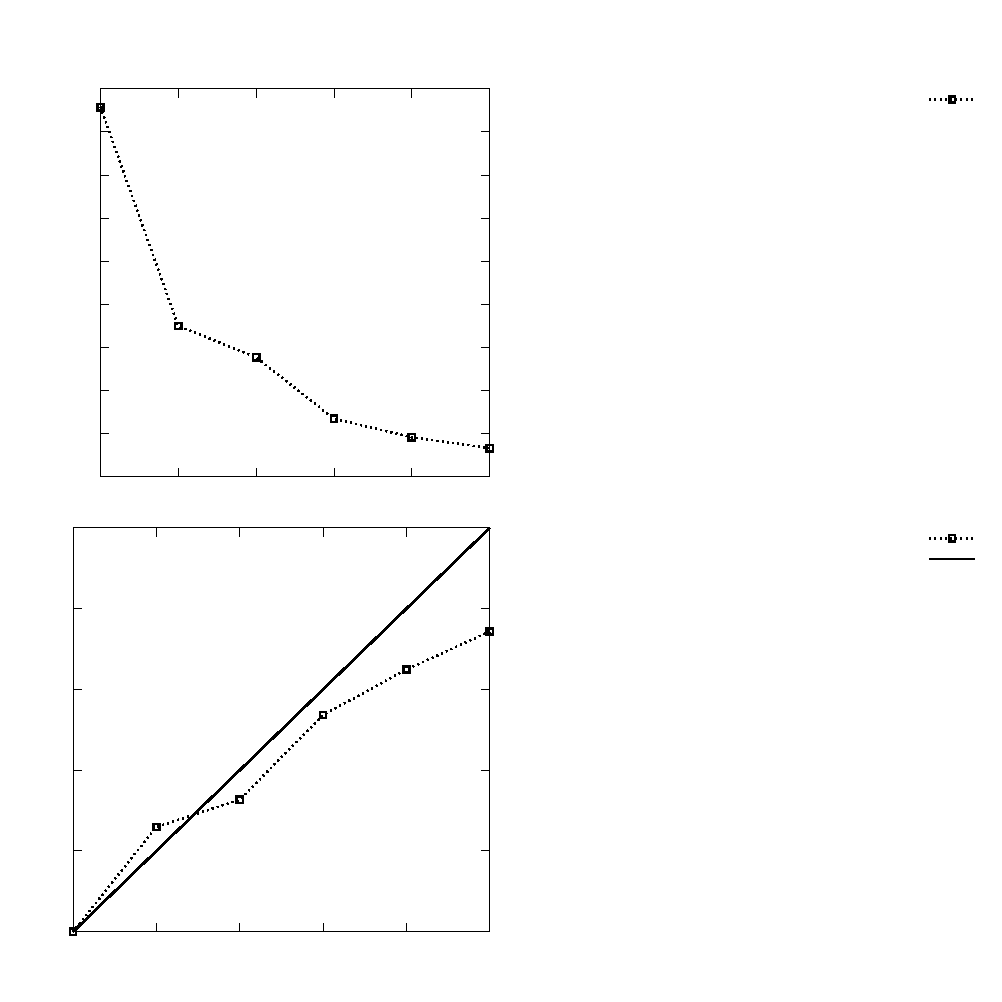
\includegraphics{MPIScalingTimes}}%
    \gplfronttext
  \end{picture}%
\endgroup
